\documentclass[11pt,letterpaper]{article}
\usepackage[T1]{fontenc}

% Titling
\usepackage{titling}
\pretitle{\raggedright\Huge}
\posttitle{\par\vspace{0.5em}}
\preauthor{\raggedright\large}
\postauthor{\par\vspace{0.5em}}
\predate{\raggedright}
\postdate{\par}

% Lists
\usepackage{enumerate}

% For mathematical documents
\usepackage{amsmath}
\usepackage{amssymb}

% Parskip
% \usepackage{parskip}
% \AtBeginDocument{\setlength{\parindent}{0pt}}

% Titlesec tiny
\usepackage[rm]{titlesec}
\titleformat{\paragraph}[runin]{\bfseries}{}{}{}[]  % Paragraph headings as run-in

% Try to kill widow lines (at top of page) and orphans (at bottom)
\widowpenalty=500
% \clubpenalty=1000

% Use endnotes
\usepackage{endnotes}
\let\footnote=\endnote


% little more space before footnote line
\setlength{\skip\footins}{1.5em plus 1em}

% it's OK to break URls on hyphens
\usepackage[hyphens]{url}
\usepackage[hidelinks]{hyperref}

% Float exactly here
\usepackage{float}
\usepackage{subcaption}
\usepackage{lscape}
\usepackage{graphicx}

% Colors
\usepackage{xcolor}

% Qframe
\usepackage{mdframed}
\newmdenv[
  topline=false,
  bottomline=false,
  rightline=false,
  skipabove=0pt,
  skipbelow=12pt
]{question}
\newcommand{\q}[1]{\begin{question}#1\end{question}}

% Outlines package
\usepackage{outlines}

% % Bibliography
\usepackage[american]{babel}
\usepackage{csquotes}
\usepackage[style=ieee]{biblatex}
\addbibresource{./bibliography.bib}


% Tabstop
\setlength{\parindent}{2em}

% Font stylings.
\usepackage{microtype}
% \usepackage{times} % Times New Roman font
% \usepackage{helvet} % Helvetica
% \usepackage{tgtermes} % TeX Gyre Termes
\usepackage{charter} % Charter

% Line spacing
\usepackage{setspace}
\onehalfspacing

% Margins
\usepackage[hmargin=1.6in,top=0.8in,bottom=1in]{geometry}

% % Crap formatting, for test
% \usepackage[margin=1in]{geometry}
% \usepackage{setspace}
% \doublespacing

\title{Detailed Design}
\author{Team 1311 | Attic ATL}
\date{\today}

%%%%%%%%%%%%%%%%%%%%%%%%%%%%%%%%%%%%%%%%%%%%%%%%%%%%%%%%%%%%%%%%%%%%%%%%%%%%%%%%%%
%% 
%%  Style guide for this document, from our profs:
%% 
%%  https://docs.google.com/document/d/1mKNSH7JZIZtfIhlVIQ8ricIseh6Ep9nLEM6A-bhde0M/edit
%% 
%%%%%%%%%%%%%%%%%%%%%%%%%%%%%%%%%%%%%%%%%%%%%%%%%%%%%%%%%%%%%%%%%%%%%%%%%%%%%%%%%%

\begin{document}

% Use lowercase roman numerals for the frontmatter page numbers
\pagenumbering{roman}

\vspace*{6em}

\newcommand{\titlelabeltext}[1]{\vspace{3em}\noindent{\color{gray}\Large{}#1}\par\vspace{0.5em}}
\newcommand{\titlebigtext}[1]{\noindent{\Huge{}#1}}

\titlelabeltext{Detailed Design of}
\noindent{}{\Huge{}OI TriageApp}\par

\titlelabeltext{Prepared For}
\noindent{}{\Large{}%
Dr. Dina Amin\\
Emory University
}

\titlelabeltext{Our Team}
\noindent{}Junior Design Team 1311\par
\vspace{0.5em}

% Table of team members
\newcommand{\email}[1]{\href{mailto:#1}{\url{#1}}}
\noindent\begin{tabular}{@{}ll}
William \textsc{Goodall} & \email{owo@gatech.edu} \\
Flynt \textsc{Wallace} & \email{uwu@gatech.edu} \\
Nick \textsc{Chapman} & \email{nchapman31@gatech.edu} \\
Ibrahim \textsc{Abotaleb} & \email{ibrahimabotaleb@gatech.edu} \\
Logan \textsc{Cyterski} & \email{lcyterski3@gatech.edu} \\
\end{tabular}

\titlelabeltext{Our Code}
\noindent\url{https://github.com/AtticATL/triage-app}

% Put the date the document was compiled on the title page.
\vfill
\noindent{\color{gray}Prepared on \today}
\vspace{5em}

% Insert a page with the table of contents
\newpage
\tableofcontents

% Insert the the list of figures
\vspace{1in}
\listoffigures

% On the next page (start of body text), switch the page numbering to arabic
% instead of lowercase roman numerals
\newpage
\pagenumbering{arabic}

\section{Introduction}
% Introduce your project, providing relevant background information (e.g. client profile, rationale for the project, project requirements etc.) and
% Provide a summary of what the Detailed Design document will cover.
% Page numbering begins with Arabic number 1
The purpose of this document as a whole is to summarize the creation of the OI Triage-App. To that end, we are Attic ATL working under the supervision of Dr. Dina Amin to make an application which will facilitate easy transfers of medical patients with OI infections between hospitals. 

\subsection{Background}
We are creating this application on behalf of our client, Dr. Dina Amin, an Associate Chief of Oral and Maxillofacial Surgery Service at Grady Memorial Hospital. Based on her experience, one of the least optimized aspects in the medical field is the act of transferring a patient and how they are dealt with on either end of the transfer. Often, these transfers are done by way of a phone call, in which it can be challenging to communicate all important details about a patient prior to transfer. This leads to situations where crucial patient information (eg. status, allergies, or more recently, COVID diagnosis) can be lost in the transfer which will place a burden on the receiving hospital's staff as they must go through the process of documenting these details once again. 

As such, the aim of this application is to create a one-stop shop which can document all of a patient's details prior to transfer and therefore alleviate the burden on the receiving hospital's staff. In order to achieve this, we will fulfill the following requirements: first, we wish to create a secure application with image, video, and data transfer capabilities. Second, we want our application to be as streamlined as possible to take the burden off of medical staff. Third, we want our application to be HIPAA compliant so it will not cause legal problems in use.  

At the conclusion of this project, we hope for a successful deployment into the hands of medical professionals, who can begin immediately using it to facilitate easy and efficient patient transfers.

\subsection{Document Summary}
As for the rest of this document, we will first cover some important terminology as well as our actual architecture and design elements in the coming sections. Following this, we will discuss how we store important data (including how we avoid violating HIPAA) and our component design, with the last important section being UI design.

\section{Terminology}

\paragraph{Triage}
The assignment of degrees of urgency to wounds or illnesses to decide the order of treatment of a large number of patients or casualties.

\paragraph{Odontegenic}
Of or relating to the formation and development of teeth.

\paragraph{Front-End} The area of development relating to the "user's side" of the application, including areas such as the user interface.

\paragraph{Patient Transfer} The process of transferring a patient from one hospital to another based off of risk and benefit analysis of the patient and each hospital's capabilities. Traditionally done through a secure telephone call as per HIPPA compliance.

\paragraph{HIPPA} The Health Insurance Portability and Accountability Act of 1960. An act that sets certain mandates that must be followed by all medical professionals to ensure patient's privacy and protection over their health information.

\paragraph{End-to-End Encryption}
A design practice where data is encrypted and decrypted locally, making it impossible for the administrators of the app to see or access user data in any way.

\paragraph{Backend}
The area of development relating to the "developer's side" of the application, including areas such as the internal database.

\paragraph{Open-Source}
A classification of software where the code to construct it is readily available to the public, allowing for easy distribution and modification.

\paragraph{JavaScript}
A programming language originally designed for websites, but now widely used across the web, mobile devices, and on the backend.

\paragraph{JSON}
A standard format for encoding structured data into machine-readable text. Stands for ``JavaScript Object Notation.''

\paragraph{React}
A free and open source JavaScript library for designing user interfaces. 

\paragraph{React Native}
A toolkit that adapts React for use on iOS and Android mobile devices.

\paragraph{Expo}
A mobile app development tool, based on React Native, that lets developers use a single codebase to target iOS, Android, and Web platforms.


\section{System Architecture}

\subsection{Introduction}
% Introduce this section by providing your reader with enough context to understand the information that follows. 
% Include the rationale behind your team’s architectural choices.

The primary constraint governing the design of our app is security. Both to comply with HIPAA, and just as good practice, all the data in our app is end-to-end encrypted. This means that, on the device of the sending ED physician, the patient profile is encrypted with a unique key. The encrypted data---called ``ciphertext''---can be freely uploaded to our backend services, because it's indecipherable without the key. The key, which in practice is a short bit of text, can be transferred to the receiving surgeon through an already-secure channel, like a phone call with a transfer center, or a URL sent over a secure messaging service. The receiving surgeon's device can fetch that ciphertext from our backend service, decrypt it with the key, and view the profile.

Because of this constraint, our app is essentially split into two halves: the sending half, responsible for filling out the profile, encrypting it, and uploading the ciphertext; and the receiving half, responsible for fetching the ciphertext, decrypting it, and displaying its data to the user.

To better understand the internal architecture of our app, we've provided both static and dynamic high-level design diagrams depicting the structural components of the application as well as how they relate to one another.


\subsection{Static Design}
% Static elements: Major architectural components are shown. Logical relationships between components are clear. There are acyclic dependencies. Style(s) are applied when appropriate. Style is correctly applied.
% Static: A structural diagram is provided that shows low-level components (classes, web pages, etc.) and their static relationships. Descriptions of functionality or attr/methods are shown. Appropriate syntax for standard diagrams, explanations for non-standard diagrams.

The figure below shows a static architectural design diagram depicting a functional view of the system, showing how different components of our app relate to one another.

\begin{landscape}
\begin{figure}
    \centering
    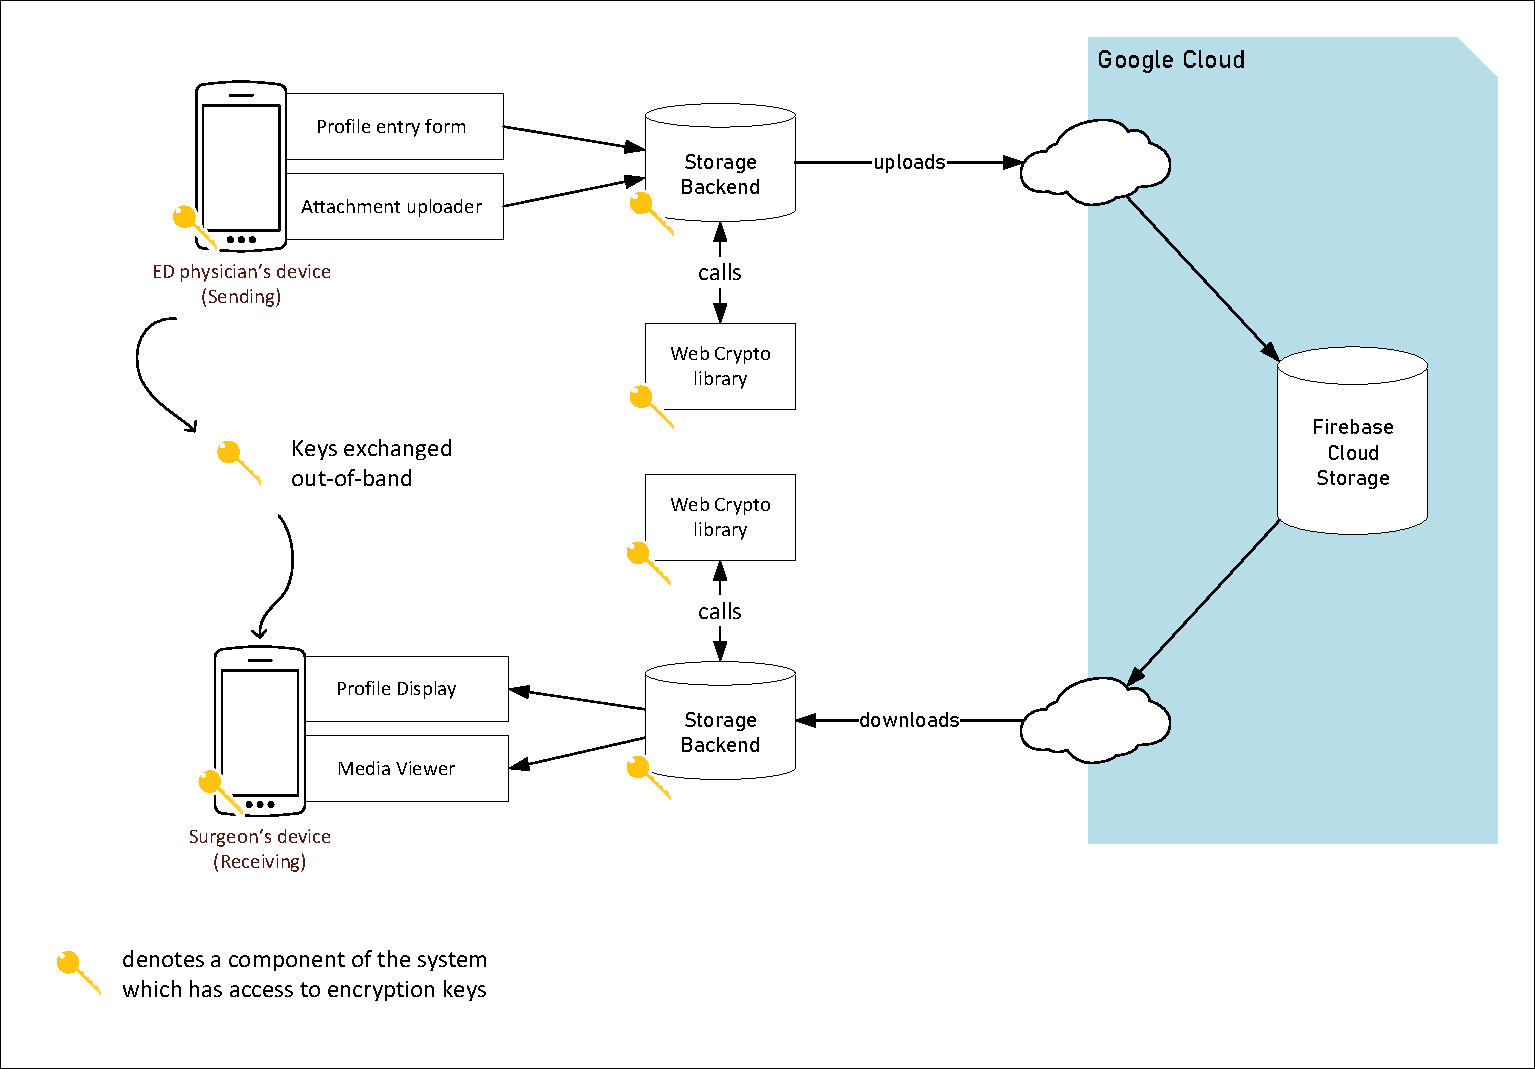
\includegraphics[width=8in]{static-design.pdf}
    \caption{Design of app components}
    \label{fig:static-design}
\end{figure}
\end{landscape}

Due to the nature of our application and its need to be compliant with HIPPA, much of the interconnected components in the background of our application deal with cryptography and ensuring that all the patient data is properly encrypted and sent. Each element of this diagram which contains a key symbol signifies that it has access to an encryption key for the current data it holds.

The first major component of our app's architecture is the front-end user portion. This mainly consists of four different systems- the profile entry form and attachment uploader for the sender and the profile display and media viewer for the receiver. These serve as the user's interface to interact with the application, with the profile entry form and attachment uploader working together to generate a profile for the patient while the profile display and media viewer serve to allow a user to see profile data on their own device. 

The second major component of our application is the storage back-end. This is where the data is encrypted and sent to the cloud for storage. Whilst sending a profile, an encryption key is generated with it. This key is sent to the web crypto library, which serves to exist as a library containing all of the keys needed to encrypt and decrypt patient data. Once these keys are stored, the encrypted data is stored in the Firebase Cloud Storage, which allows us to store mass amounts of data while being HIPPA compliant as the data stored is all encrypted and unreadable until an app containing the keys decrypts it. 

\subsection{Dynamic Design}

The dynamic architecture design system sequence diagram provides a look at the two main control flows of our application and how they interact with the different components of the application. Figure 2 depicts the control flow of a user sending a patient profile to the cloud, and Figure 3 depicts the control flow of a user recieving a patient profile from the cloud. 

% Dynamic: A diagram is provided that shows runtime interactions of the static components. Appropriate diagram is chosen. Behavior illustrates how system will operate on a non-trivial use case.
% Dynamic elements: A scenario or SSD is provided to show runtime behavior. Components interact logically and in accordance with style chosen.

% Edit the SSD at:
% https://swimlanes.io/u/yM7aQAwsB

\begin{landscape}
\begin{figure}
    \centering
    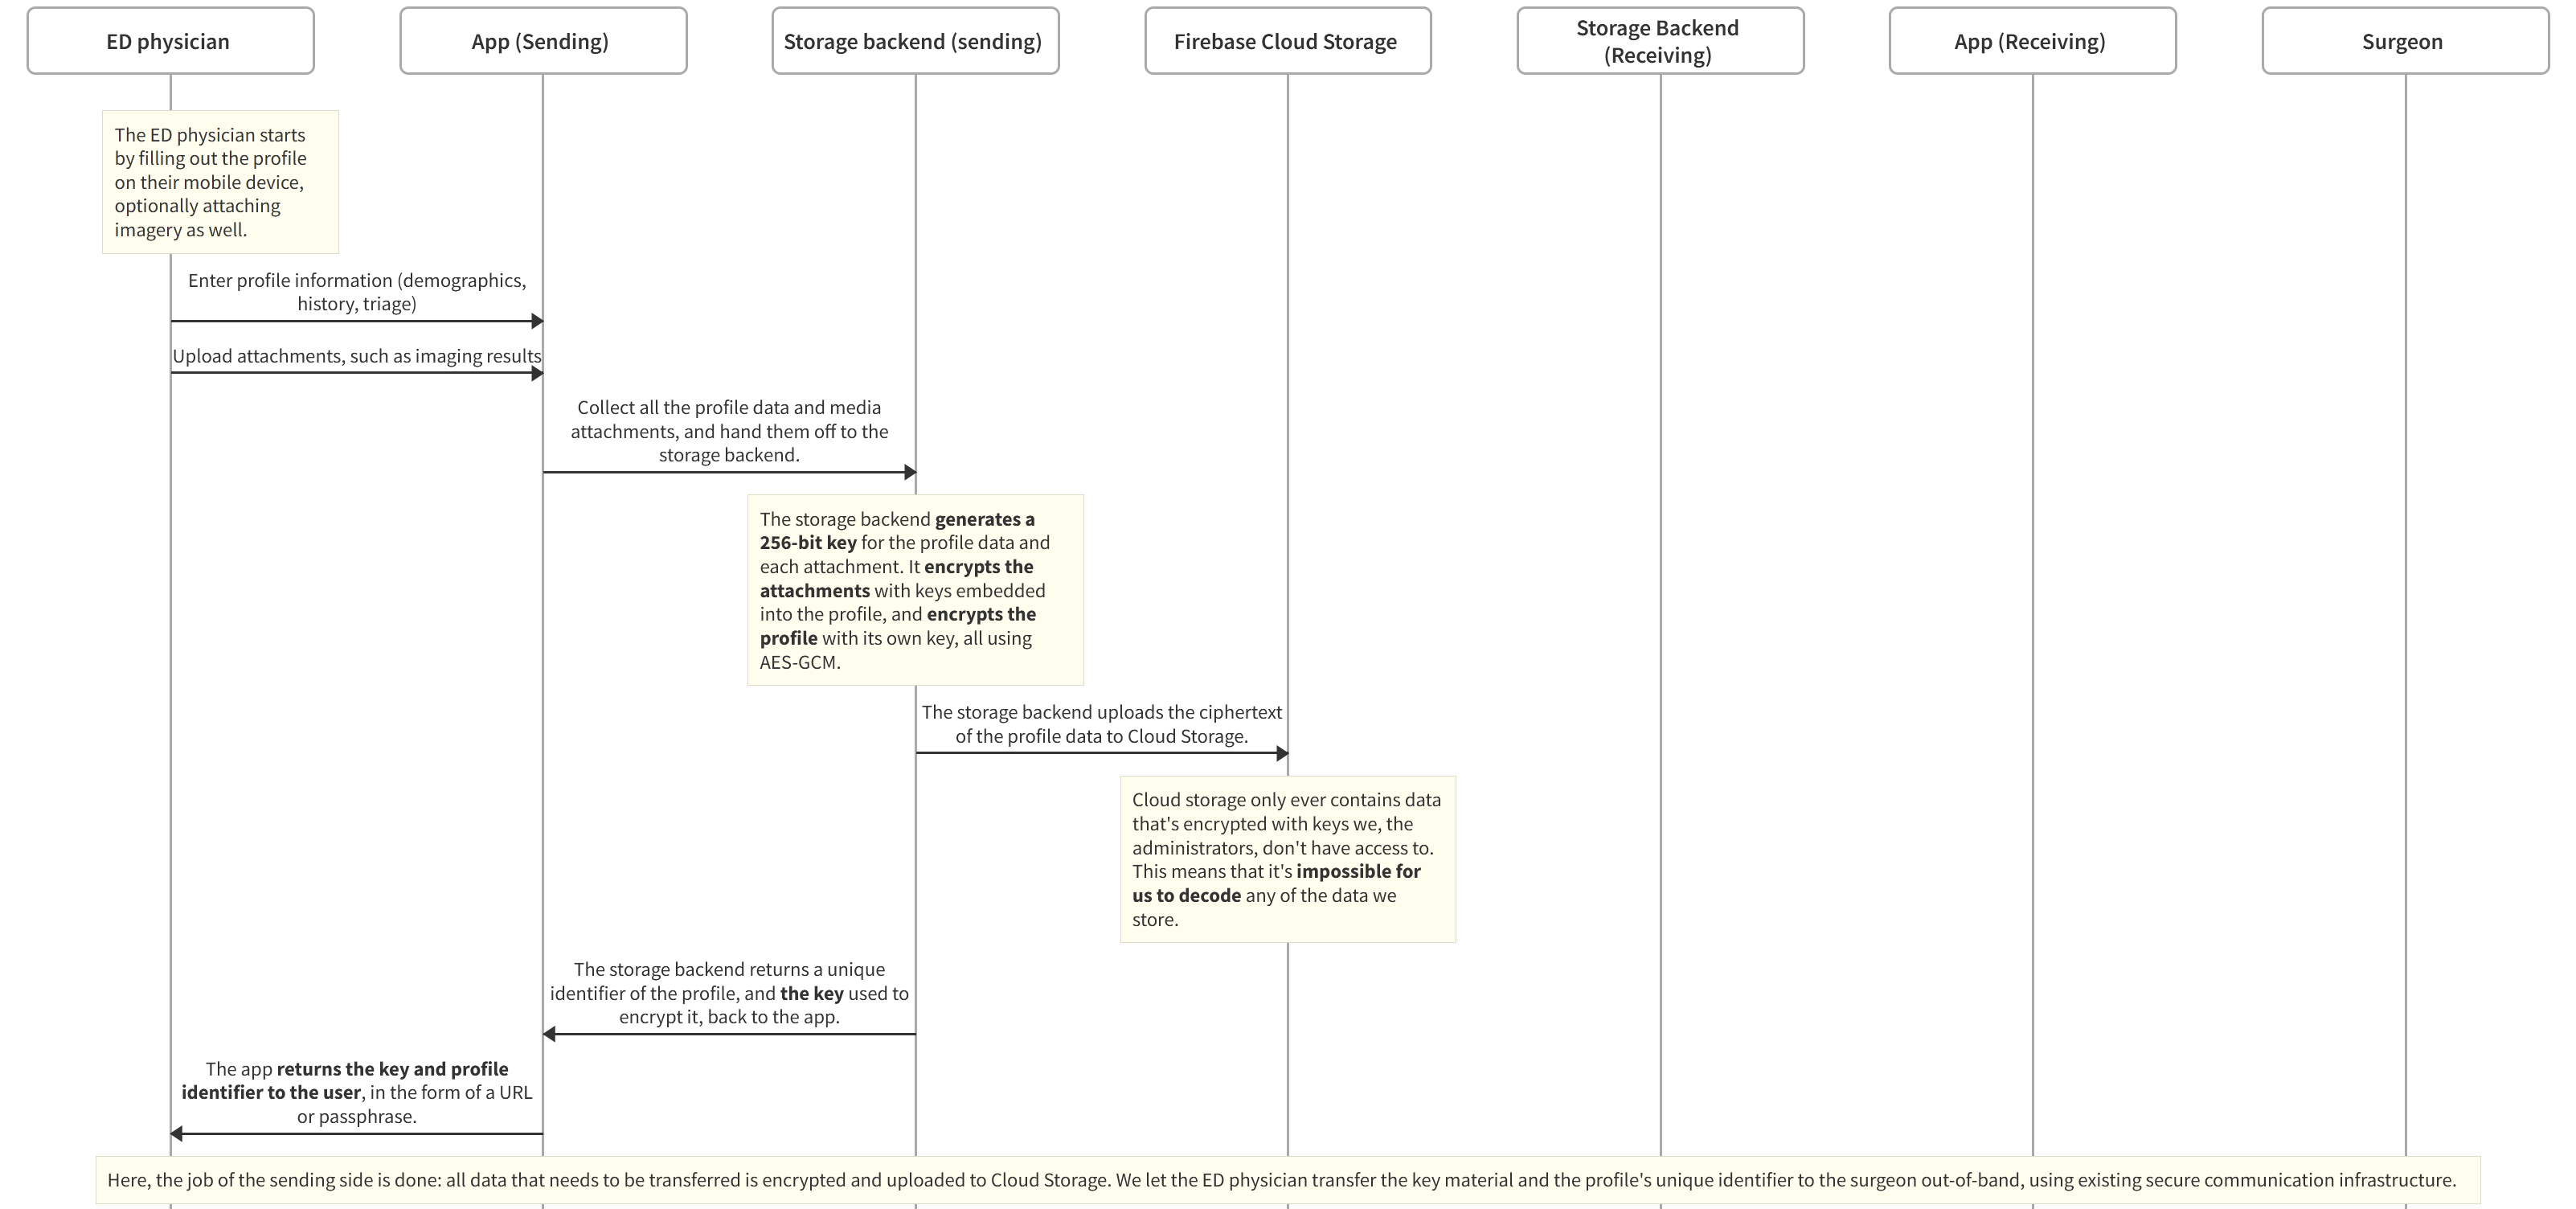
\includegraphics[width=9in]{sequence-diagram-1.png}
    \caption{Sequence of events to encrypt and send a profile}
    \label{fig:sequence-1}
\end{figure}
\begin{figure}
    \ContinuedFloat
    \centering
    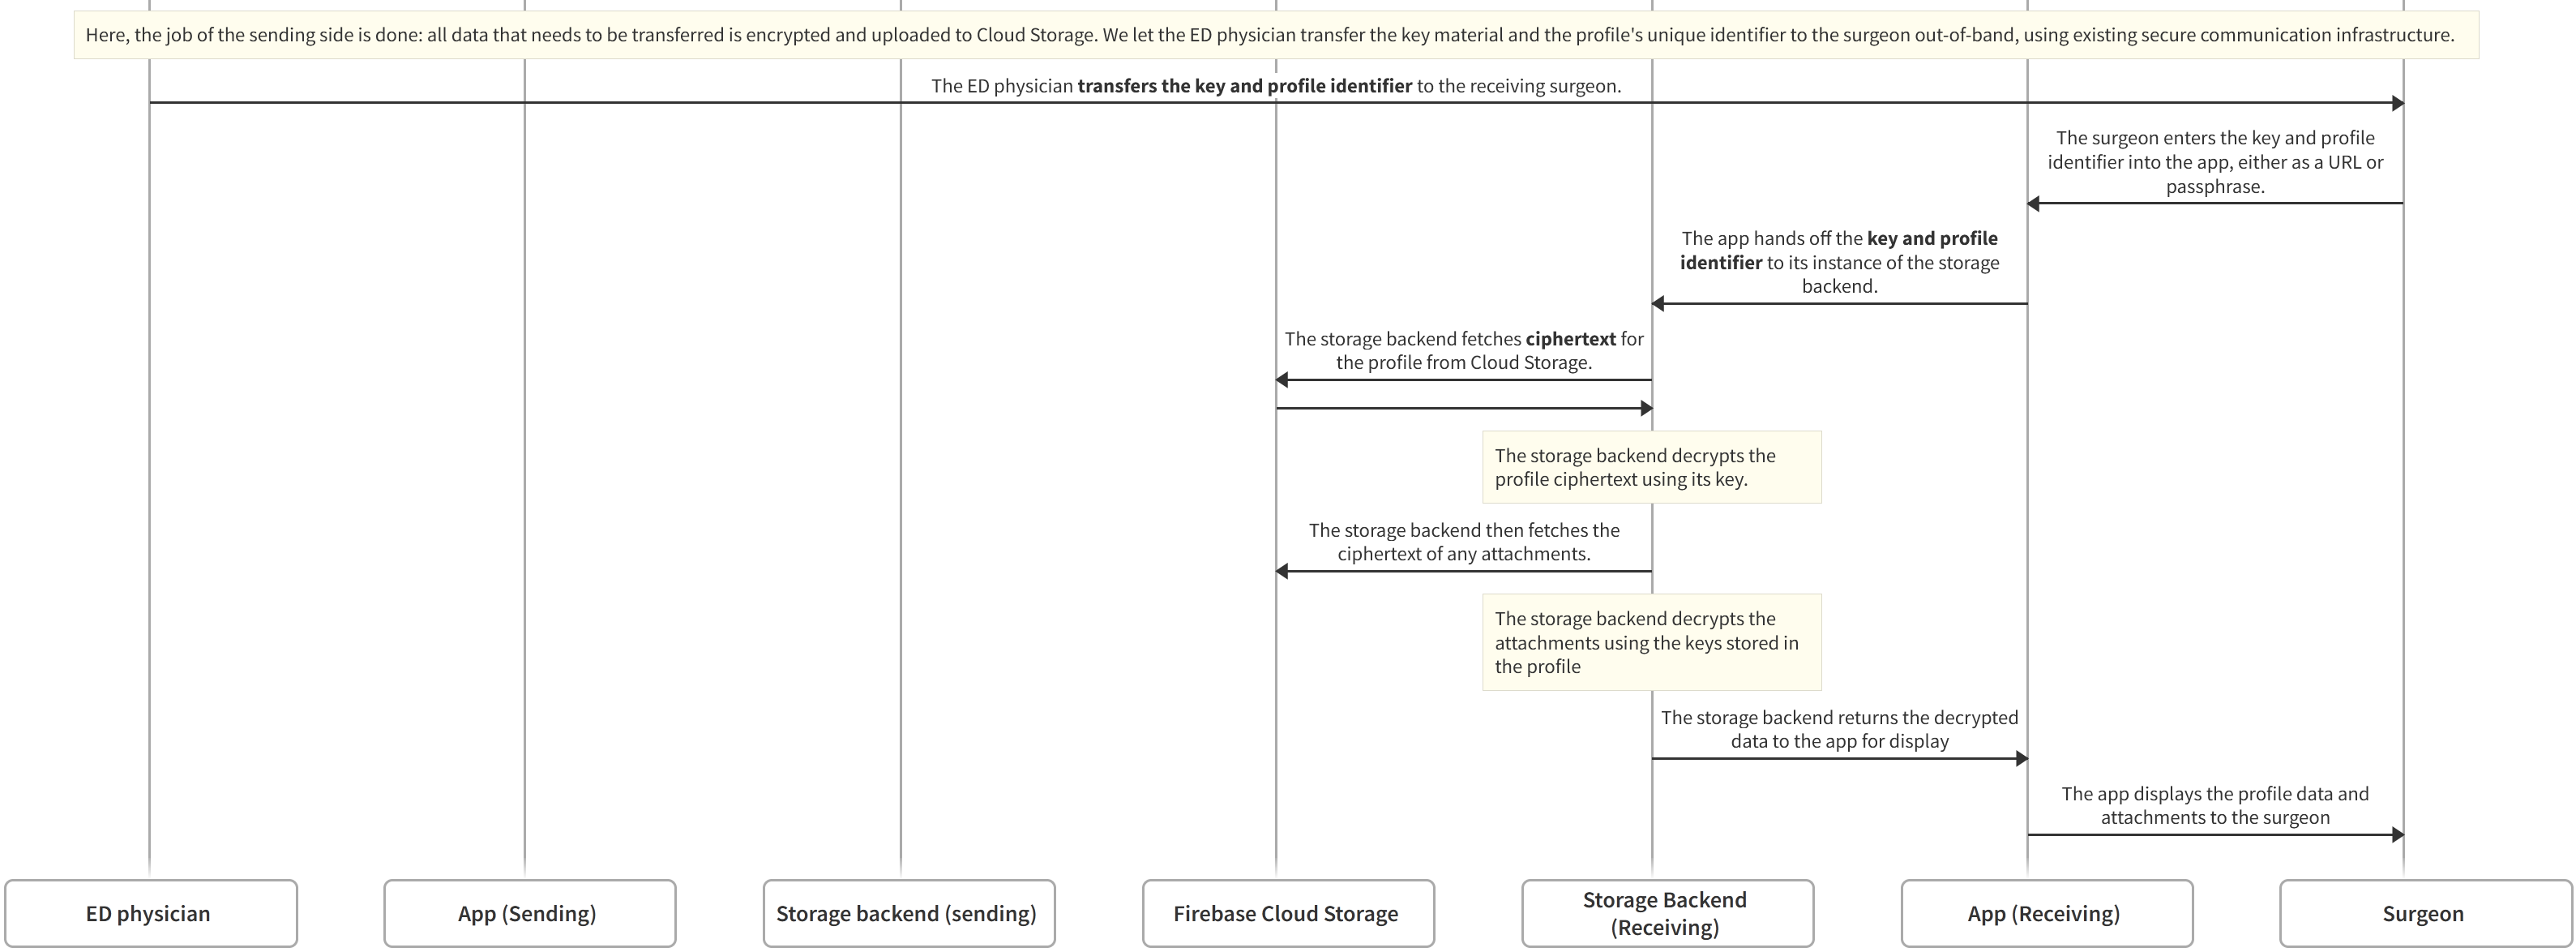
\includegraphics[width=9in]{sequence-diagram-2.png}
    \caption{Sequence of events to decrypt and receive a profile}
    \label{fig:sequence-2}
\end{figure}
\end{landscape}

\section{Data Storage}
% For database use: An ER diagram is provided. Relationships between tables and cardinality constraints are shown. Tables are appropriately normalized. PK/FK relationships are shown if needed.
% For file use: Format is documented if non-standard. Otherwise, a standard format is chosen.  
% For data exchange: Format is documented.

The data storage needs for this app are not particularly complex: we need to be able to store a few fields of data that represent a patient profile (name, date of birth, triage information, etc), and we need to be able to store media attachments to that profile (like images). However, we are subject to a few significant constraints, which impose extra complexity on our implementation.

The first constraint is security. All data should be end-to-end encrypted, and inaccessible to the operators of the app's backend. This rules out using a traditional architecture, where we would host a single database server behind some application code to perform logic and enforce access control. To solve this, we encrypt all application data on the device before it gets sent to our backend---and the only thing our backend can see is blobs of ciphertext.

The second constraint is portability. Data needs to be transferable between instances of the app, even if those instances are running slightly different versions. To solve this, we're using a schema to strictly define the shape of our data, so that an instance of the app receiving data knows exactly what it's going to get.

Our implementation, taking in mind our objectives and constraints, is based on an encrypted, globally-synced key-value store. This store implements two operations---\verb|get| and \verb|put|. The \verb|put| operation takes some data, encrypts it, stores the ciphertext in cloud storage, and returns a handle: composed of a unique identifier for that data, and the key required to decrypt it. The \verb|get| operation does the reverse: it takes a handle, uses it to fetch the right data from cloud storage, and returns the plaintext back to the caller.

When a user uses the app, they fill out a profile---which is represented internally as a JSON object conforming with our schema---and select media from their device to be included as attachments. Each media attachment is stored in the key-value store (using the \verb|put| operation). The handles for each attachment are stored in the profile JSON. Once all the attachments are encrypted and uploaded, we store the full profile in the key-value store as well. The handle for the profile can then be transfered between devices out-of-band. 

Because these data handles contain key material, a receiving app can use a handle it gets from a user to fetch and decrypt a profile. This profile will contain handles for any media attachments which have been included---which the app can fetch and decrypt as well. Once the receiving side has done this, it has all the information it needs to present the profile to the user.

We've specified the format of the profile data in code with a schema. This helps to catch any bugs involving the data format, because the same functionality that checks user input for correctness (e.g. that birth dates must be in the past) will also check the app's code for correctness (e.g. a typo on a field name, or leaving a value \verb|null| when it should be defined). The source code defining the schema is included as appendix \ref{appendix:profile}.


\section{Component Design}

\subsection{Introduction}

In this section,we will be going over the general design of the application as we did in the system architecture section, but this time taking a more in-depth look as to the individual class components that make up the application. Using both a static component diagram and a dynamic system sequence diagram, we aim to better represent the interactions and relationships of the internal components that make up our application.

\subsection{Static Diagram}

The component diagram below designates a static view of the different components of our application, clarifying hierarchies, ownership, and designed associations.

\begin{landscape}
\begin{figure}
    \centering
    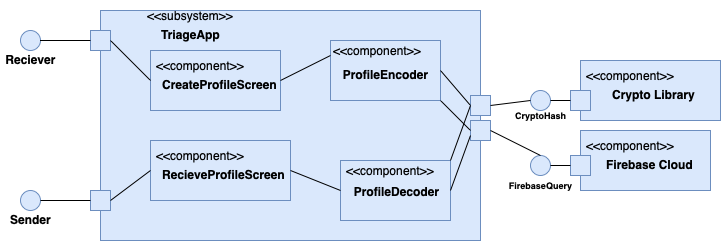
\includegraphics[width=8in]{component.png}
    \caption{Component diagram of application's interactions}
    \label{a}
\end{figure}
\end{landscape}

The TriageApp subsystem makes up the majority of our application. This includes two sets of components for each of the two main functions of our application- a CreateProfileScreen that accesses its subsequent ProfileEncoder for the sending party, and a RecieveProfileScreen that accesses its subsequent ProfileDecoder for the receiving party. Both components use the ports outside of the TriageApp, produce a cryptography hash, and Firebase query respectively to get/store the cryptography keys and the associated data. It can be clearly seen that the application design is very parallel, as every encoding feature has it's appropriate decoder, and each use case get it's own separate screen to maximize utility for that specific user.

\subsection{Dynamic Diagram}

The sequence system diagram shown below designates a trace through the flow of our application from the perspective of a sender creating a patient profile and sharing it. 

\begin{landscape}
\begin{figure}
    \centering
    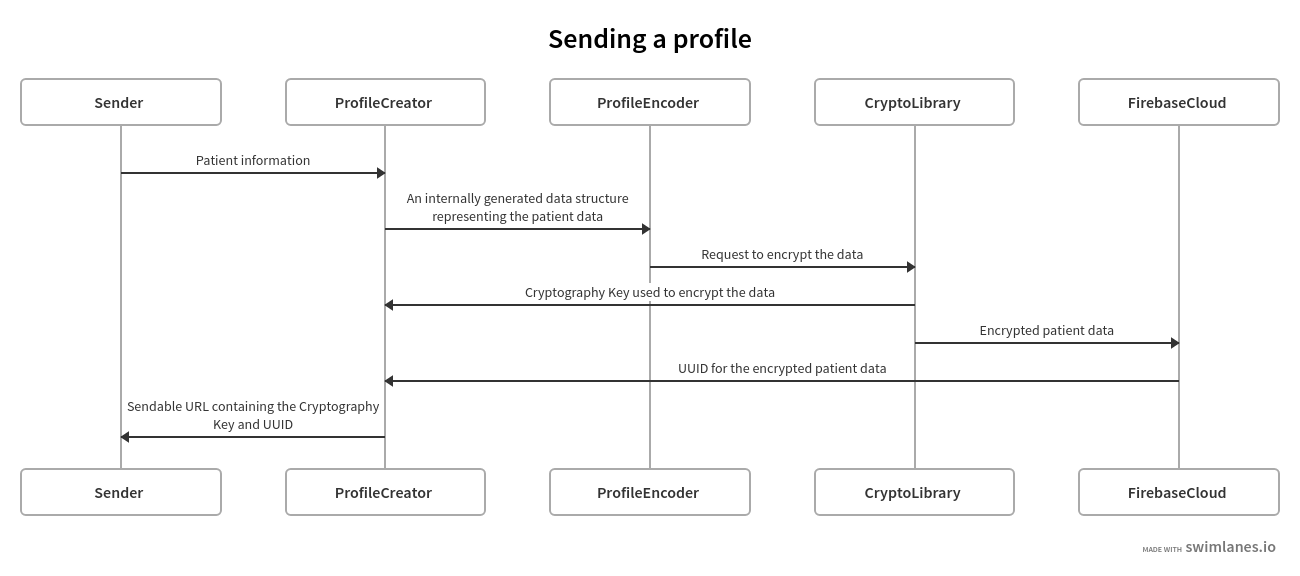
\includegraphics[width=8in]{component-sequence.png}
    \caption{Component diagram of application's interactions}
    \label{a}
\end{figure}
\end{landscape}

The sequence begins by having the sender create the patient profile by transferring all of the relevant patient data into the ProfileCreator through the use of the triaging checklist, text fields, and image uploads associated with the screen. This profile data is then subsequently sent to the profile encoder, which prepares all of the data to be encoded and sends a request to encode the generated patient data. The CryptoLibrary then proceeds to encrypt the patient data given to it, returning a key back to the user as well as pushing this data forward to the Firebase Cloud for storage. 

Once the encrypted data is stored in the Firebase Cloud, a UUID related to the patient profile is then generated and sent back to the profile creator. The profile creator then finally takes the cryptography key from the crypto library and the UUID from the Firebase Cloud and combines them into a send-able URL so that a receiving party will be able to access the data through the UUID and decrypt it through the cryptography key. 

\section{UI Design}
% Major screens are provided.  
% Widget selection and layout which is appropriate and logical  
% Proper UI design principles are applied to the screen design.



% % Insert Bibliography
% % Note: we're required to use IEEE style here
% \clearpage
% \nocite{*}
% \printbibliography[title={References}]

\newpage
\vspace*{2in}\noindent{}{\Large{}Appendices}
\newpage
\begin{appendices}

\section{Profile Schema Definition}
\label{appendix:profile}

Here, we list the source code used to define the shape of a patient profile. We use the \verb|zod| library for TypeScript, which gives us detailed runtime checks for user-visible feedback (e.g. an invalid date field), as well as compile-time checks for programming errors.

\inputminted{typescript}{profile.ts}



\end{appendices}

\end{document}